%!TEX root = ../dissertation.tex
\begin{savequote}[75mm]
This is some random quote to start off the chapter.
\qauthor{Firstname lastname}
\end{savequote}

\chapter{Electronic cooling mechanisms in graphene}
\label{ch:electronic_cooling}
\newthought{Charge carriers in conductors} exchange energy with the environment in many ways. If an electronic system is directly heated --- whether it be by Joule heating, optical pumping, and any other direct energy transfer --- the mechanisms with which the system cools can be quite diverse. In mesoscopic samples there are typically three cooling mechanisms one has to consider. First, if the material is electrically connected to a thermal bath, such as macroscopic electrodes, then hot electrons can diffuse out and cold electrons can diffuse in; this diffusion is often referred to as Wiedemann-Franz cooling and is the dominate thermal transport mechanism in metals at low temperature~\cite{kittle??}. Secondly, hot electrons can transfer energy directly to the lattice by coupling to acoustic and optical phonon modes in the graphene itself or the nearby substrate~\cite{??}. Thirdly, electrons are charged and can therefore radiatively cool; this radiation is often in the form of Johnson noise and, although often negligible even at cryogenic temperature, can be the dominate cooling mechanism in ultra-sensitive bolometers~\cite{prober, mckitterick}.


\section{Wiedemann-Franz}
First observed at room temperature in 1853 by Wiedemann and Franz~\cite{franz_ueber_1853},  the thermal conductivity, $\kappa$, of metals is directly proportional to the electrical conductivity, $\sigma$, at room temperature. Twenty years later, Lorenz expanded upon the idea and showed the ratio of the thermal conductivity to the product of the electrical conductivity and temperature, $T$, was a constant~\cite{lorenz_bestimmung_1872}, $\sL$.
\begin{equation}\label{eq:WF}
\frac{\kappa}{\sigma T} = \sL
\end{equation}
Eq.~\ref{eq:WF} is now known as the Wiedemann-Franz law (WFL) where $\sL$ is the Lorenz ratio. Data showing experimentally measured Lorenz numbers for various metals and semi conductors as a function of conductivity and carrier concentration is shown in fig.~\ref{fig:WF_in_metals}.
\begin{figure}
\centering
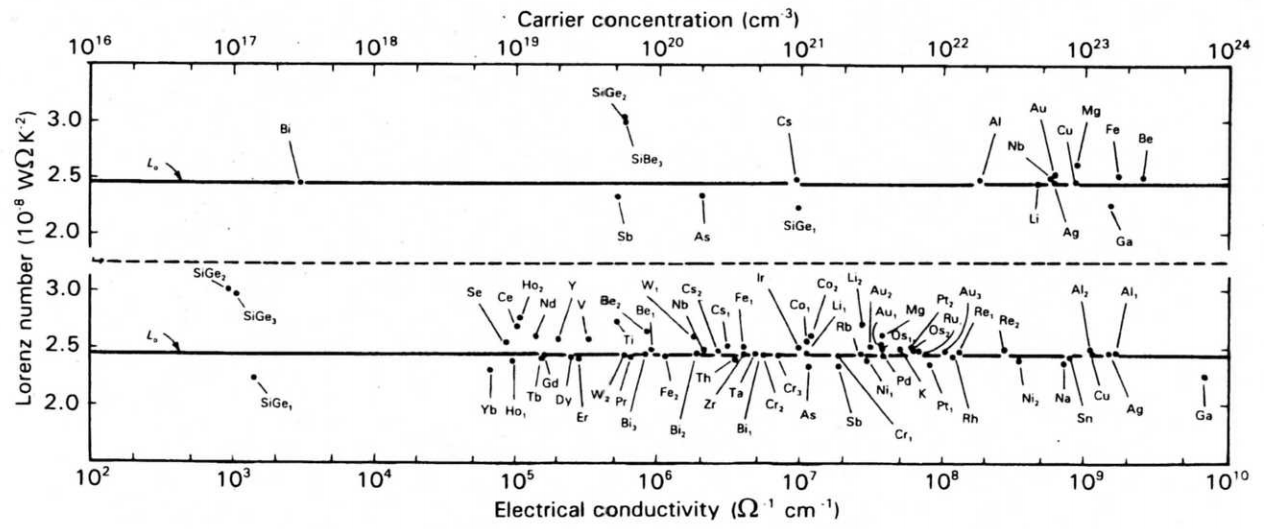
\includegraphics[width=\textwidth]{figures/electronic_cooling/WF_in_metals.png}
\caption{Experimental Lorentz number of elemental metals and degenerate semiconductors at low temperature. Taken from ref~\cite{kumar_experimental_1993}. \textit{reprinted with permission, Springer, license number 4067330556225}}
\label{fig:WF_in_metals}
\end{figure}
The quantitative value for $\sL$ can be derived approximated under the Drude model~\cite


basic mechanism. Electron carry heat away through conduction. Each particle carries a fixed charge and fixed heat capacity. Include equation. Discuss assumptions. Show plot of experimental agreement.

\subsection{Linearization}

\subsection{Hot electron shot noise}

\section{Electron-Phonon coupling}
general form including delta and Sigmaelph.

\subsection{Linearization}

\subsection{Bloch-Gruneisen temperature}

\subsection{Acoustic phonon}

\subsection{Intrinsic optical phonons}

\subsection{Remote optical phonons}
include some table keeping track of the power laws

\section{Photon cooling}
This is Johnson noise and its what you measure

\section{Heat transfer equations}
total heat transfer for the entire system Q=…
formulate kappa equations for general steady state heating profile
